\section{Regime-Switching Fair Value (Realized Volatility vs VIX)}

\IfFileExists{generated/regime_switch_metrics.tex}{%
  % Generated by analyze_icma_dataset (plot_regime_switch_sensitivity).
\providecommand{\RegimeSwitchBestModelBase}{RatesVolEquity\_d}
\providecommand{\RegimeSwitchBestModelReg}{RatesVolEquity\_d}
\providecommand{\RegimeRVColumn}{S\&P}
\providecommand{\RegimeSwitchRsqOut}{0.5973}
\providecommand{\BaselineStaticRsqOut}{0.6978}
\providecommand{\RegimeSwitchDeltaRsq}{-0.1006}
\providecommand{\RegimeSwitchRmseOut}{1.8480}
\providecommand{\BaselineStaticRmseOut}{1.6007}
\providecommand{\RegimeVolWindow}{21}
\providecommand{\RegimeSignalThreshold}{3}
%
}{%
  \providecommand{\RegimeSwitchBestModelBase}{---}%
  \providecommand{\RegimeSwitchBestModelReg}{---}%
  \providecommand{\RegimeRVColumn}{S\&P}%
  \providecommand{\RegimeSwitchRsqOut}{---}%
  \providecommand{\BaselineStaticRsqOut}{---}%
  \providecommand{\RegimeSwitchDeltaRsq}{---}%
  \providecommand{\RegimeSwitchRmseOut}{---}%
  \providecommand{\BaselineStaticRmseOut}{---}%
  \providecommand{\RegimeVolWindow}{---}%
  \providecommand{\RegimeSignalThreshold}{3}%
}

\subsection*{Motivation}

The static fair-value models in the main report assume a single linear mapping
from daily changes in drivers to \(\Delta\)CDX IG. As an alternative
\textbf{sensitivity} (not used in the main PDF pipeline), we allow the OLS
coefficients to depend on a simple \emph{volatility regime}: at each date,
one-month trailing realized volatility of the S\&P index level (from daily
percentage changes, annualised, in percentage points) is compared to the VIX
level. When realised volatility
exceeds VIX by more than \RegimeSignalThreshold{} percentage points on the
annualised spread (same units as the plot), we label the day
regime~1; otherwise regime~0. Each candidate model is still evaluated on the
same chronological train/test split, but within the training window separate OLS
fits are used for observations in each regime when enough points are available.

\subsection*{Out-of-sample performance}

For the selected best specification, out-of-sample \(R^2\) is
\BaselineStaticRsqOut{} under a single pooled OLS on the training window versus
\RegimeSwitchRsqOut{} under the regime-switching estimator (difference
\RegimeSwitchDeltaRsq{}). RMSE on the test set is
\BaselineStaticRmseOut{} versus \RegimeSwitchRmseOut{} respectively. The best
model name is unchanged (\RegimeSwitchBestModelReg{}) in this sample.

\subsection*{Timing of regime changes}

\begin{figure}[H]
  \centering
  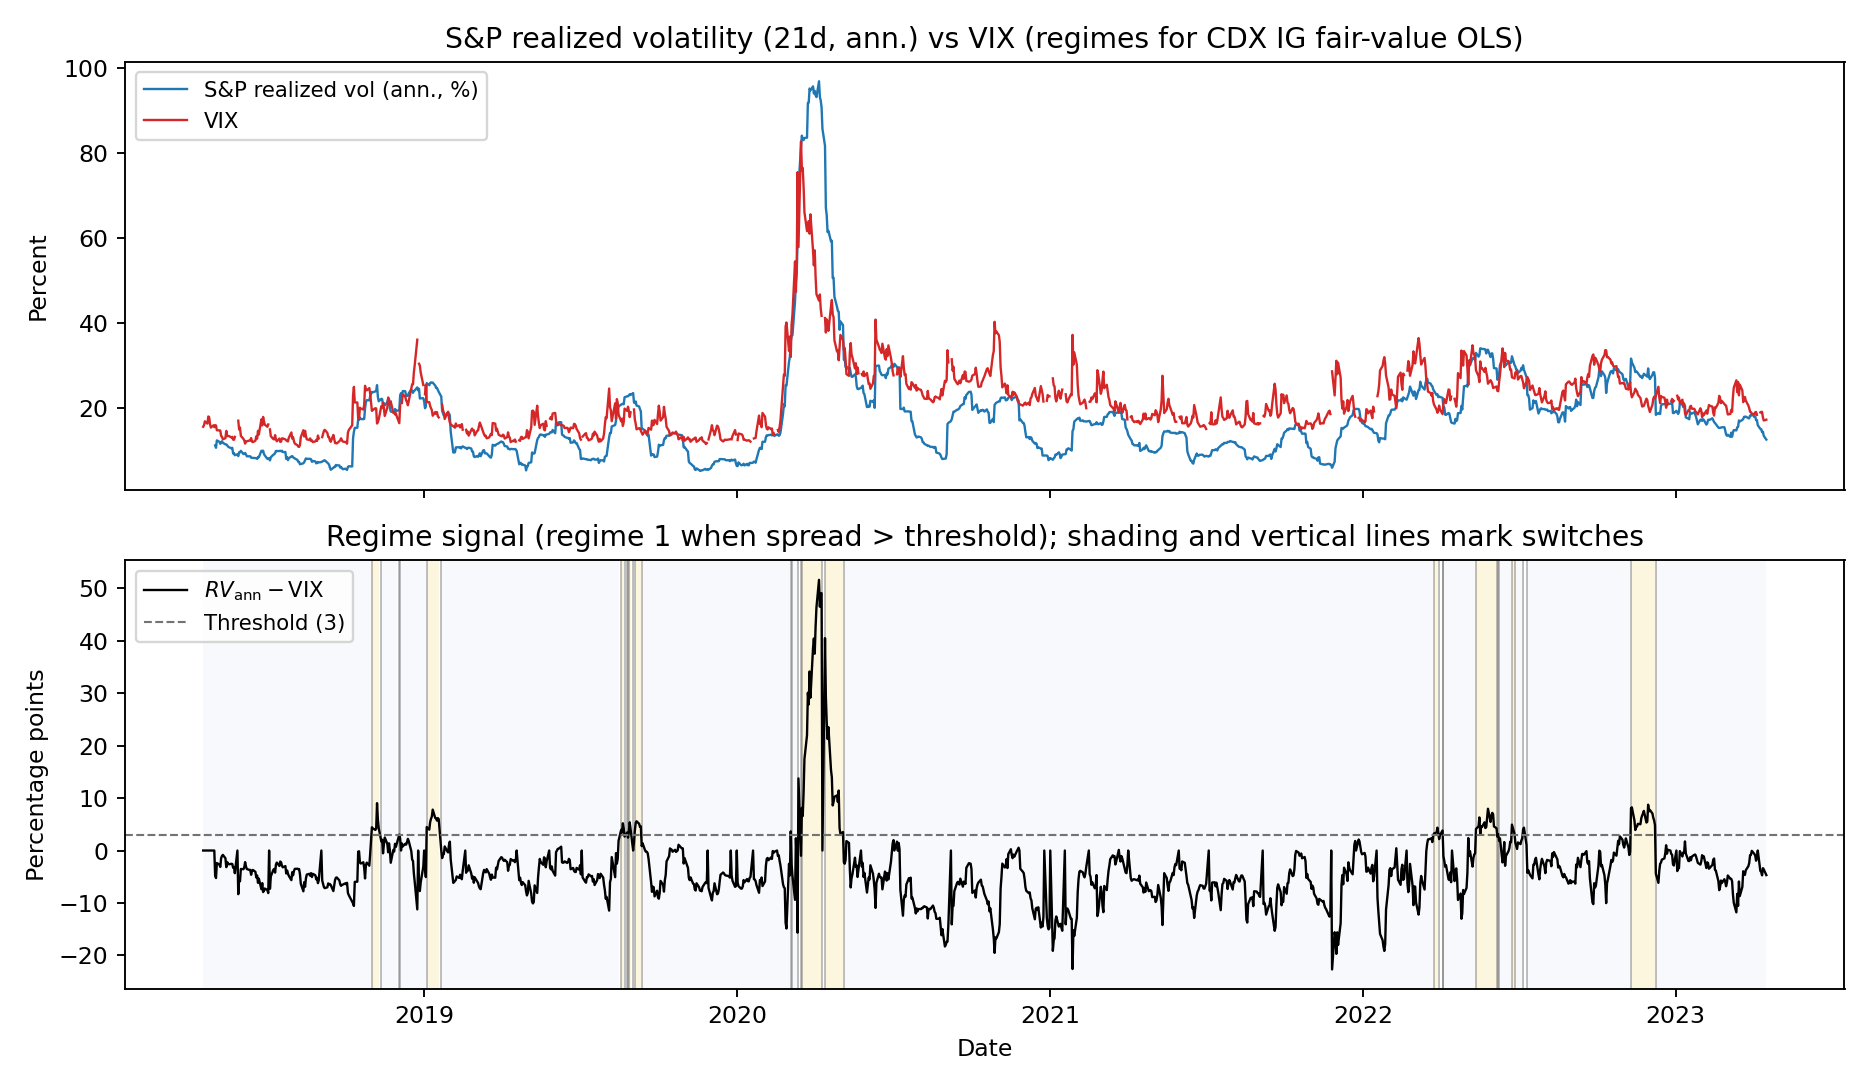
\includegraphics[width=\textwidth]{../../../output/figures/CDX_IG_regime_rv_vix.png}
  \caption{\textbf{Top:} \RegimeRVColumn{} realised volatility
    (\RegimeVolWindow{}-day window, annualised) and VIX.
    \textbf{Bottom:} spread \(RV_{\mathrm{ann}}-\mathrm{VIX}\) vs threshold~\RegimeSignalThreshold{}.
    Shading: regime~1 in \emph{yellow} tones, regime~0 in a \emph{light grey}
    background; vertical lines mark regime switches. Same regime rule as in the
    Motivation for CDX IG fair-value OLS.}
  \label{fig:regime_rv_vix}
\end{figure}
\FloatBarrier
\clearpage

Figure~\ref{fig:regime_fair_value_levels} overlays realised CDX IG with fair
value from the \emph{same} best specification (\RegimeSwitchBestModelBase{}):
pooled static OLS versus regime-switching OLS (per-regime training fits when
enough observations are available, as in the Motivation).

\begin{figure}[H]
  \centering
  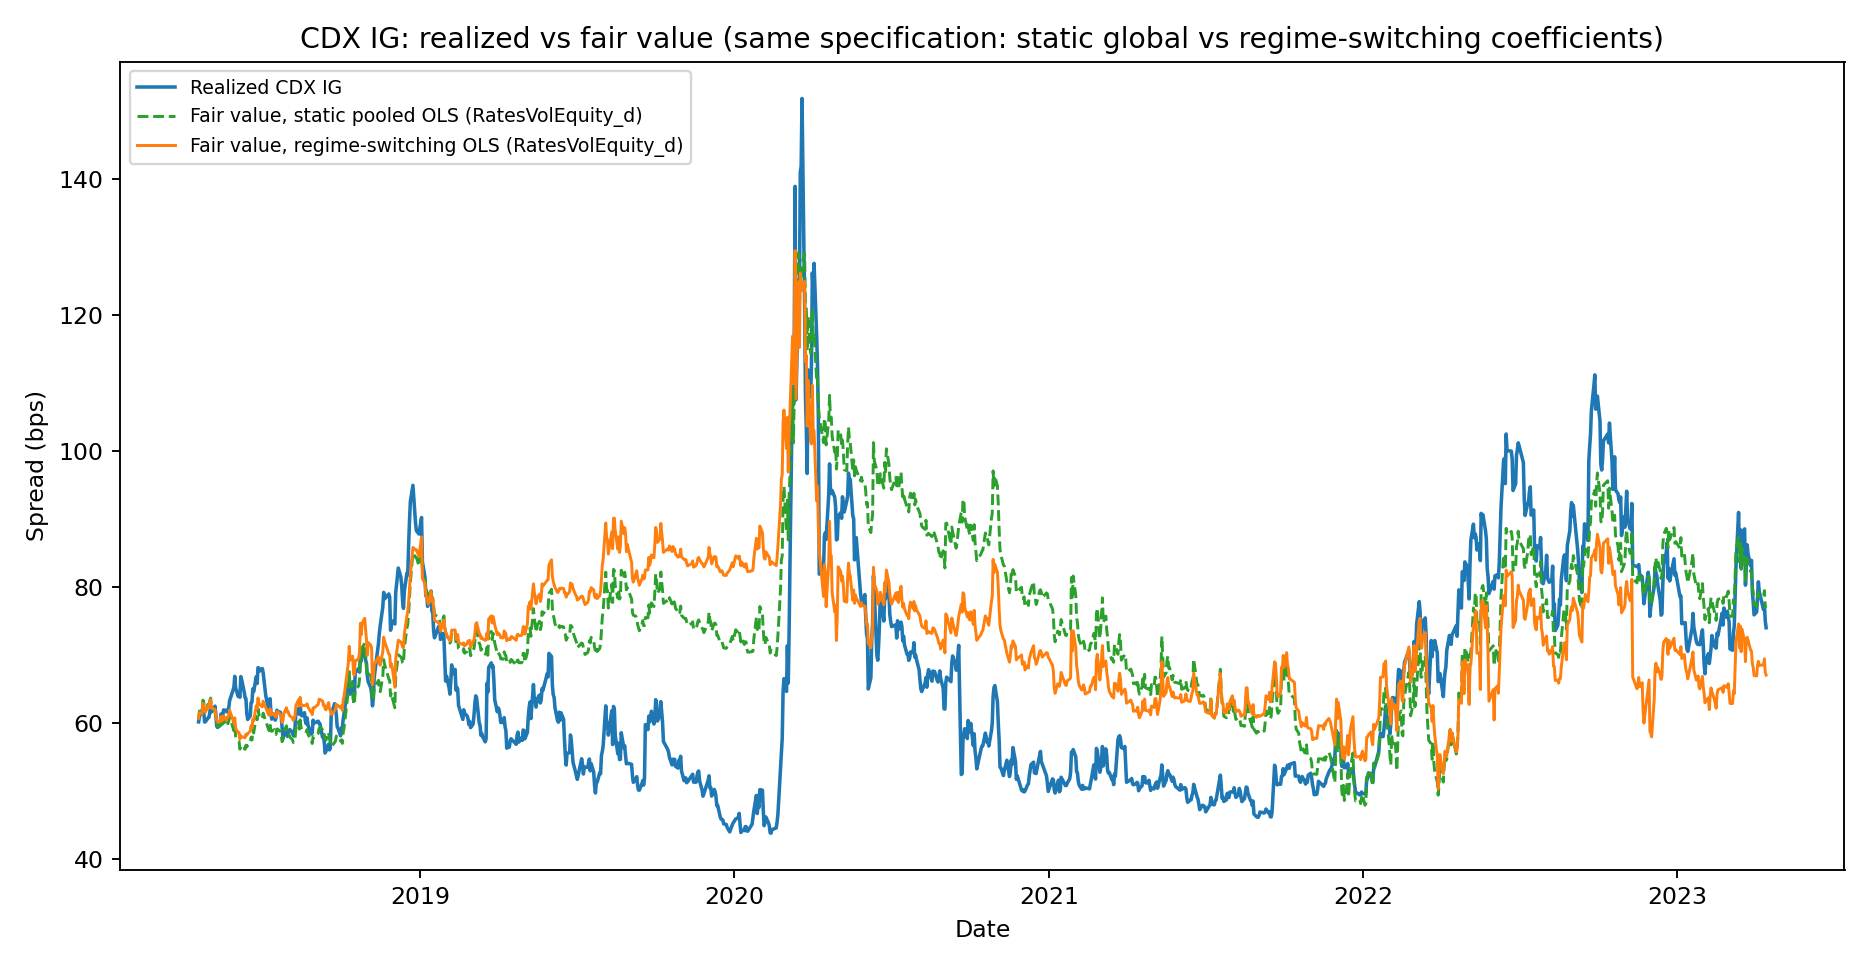
\includegraphics[width=\textwidth]{../../../output/figures/CDX_IG_regime_vs_static_fair_value.png}
  \caption{Realised vs.\ fair CDX IG for the best static specification:
    pooled OLS (global coefficients) and regime-switching OLS (per-regime
    coefficients when subsamples are large enough).}
  \label{fig:regime_fair_value_levels}
\end{figure}
\clearpage

The regime-switching specification does not replace the main static model; it
illustrates how conditioning on an equity-index volatility gap (S\&P RV vs VIX)
can be incorporated without altering the rolling-window machinery used
elsewhere in this document.
